\section{Introduction}

Gaia \citep{Prusti2016} released sparse photometry for about 157{,}000 numbered asteroids in DR3
\citep{Vallenari2023,Tanga2023}. Sparse photometry can constrain periods and spin states
\citep{Kaasalainen2004}, and three groups have derived rotation periods and poles from DR3
\citep{Durech2023,Cellino2024,MacLennan2026}. \citet{Durech2023} estimated a false-solution rate of about
0.6\% against LCDB periods of quality $U=3$. That rate refers to asteroids with a reliable published period.
For an asteroid that has no published period, the rate is not known, and it is the rate a user of a new
period needs.

This paper sets out to measure it and to deliver the products that depend on it. The reliability of each
period is calibrated on one half of the LCDB, tested on the other half, and bounded by null tests that keep
the real Gaia sampling. The paper then gives:
(i) for 6{,}238 asteroids, a period with a tested probability of being correct, 1{,}680 of them absent from
all three earlier DR3 analyses;
(ii) a spin sense for each of them, 1{,}447 for asteroids with no pole in six pole catalogues, checked
against independent ATLAS poles;
(iii) 39 LCDB periods that disagree with independent survey data, and 69 more flagged by agreement among
Gaia DR3 analyses;
(iv) 790 candidate new periods, with their noise and alias rates.
The pipeline runs on all of DR3 in about 20 minutes on a laptop with ten processes, so it can be rerun as
soon as Gaia DR4 is released. A pilot on 600 asteroids was reported in \citet{Tropynin2026a}.

\section{Data and geometry}

All 20 bulk files of \texttt{sso\_observation} (23.3\,M CCD rows) were averaged per \texttt{transit\_id}.
This gives 3{,}069{,}170 transits of 156{,}789 numbered asteroids, of which 42{,}195 have at least 25
transits. Each transit carries the largest relative flux error of its CCDs, a conservative choice that
covers CCD-to-CCD scatter, added in quadrature to a 0.03\,mag floor. A season is a run of transits with no
gap longer than 60\,d. Before the search, transits deviating from a fit of season offsets and a phase term
by more than $5\times1.4826$ times the median absolute deviation are removed, and the cut is repeated once;
353 asteroids then fall below 25 transits and are dropped.

Heliocentric positions come from JPL osculating elements (epoch 2026 June), integrated back to 2014--2017
with a fourth-order Runge--Kutta scheme and a one-day step, with the four giant planets as perturbers. Gaia's
position is taken from the data, and light time is iterated. Against JPL Horizons on 19 asteroids, the
reduced magnitudes differ by at most 0.0007\,mag.

The analysis code was written with the help of a generative AI assistant (Claude, Anthropic) under the
author's direction. Its output was checked independently of the code: against JPL Horizons as above, by
the held-out TEST half, the null tests, the injections, and comparison with independent surveys. The code is
public (see Data availability).

\section{Model and search}\label{sec:model}

The reduced magnitude $G-5\log_{10}(r\Delta)$ is fitted by weighted least squares with one constant per
observing season, a term linear in phase angle, and a second-order Fourier series in the phase
$2\pi(ft-s\,\lambda_{\rm PAB}/360^\circ)$. Here $\lambda_{\rm PAB}$ is the ecliptic longitude of the
phase-angle bisector seen from Gaia \citep{Harris1984} and $s=\pm1$ is the sense of rotation. Both senses
are searched and the better fit is kept. The correction is exact for a pole at the ecliptic pole, so the
periods are approximately sidereal.

Over a season $\lambda_{\rm PAB}$ advances almost linearly, and a linear advance is equivalent to a small
shift of frequency, the same for both senses up to sign. The sense is therefore constrained by the
non-linear part of $\lambda_{\rm PAB}(t)$ across seasons, and only when the pole is far from the ecliptic;
Section~\ref{sec:spin} shows how the accuracy depends on pole latitude.

The search covers periods of 2--1000\,h on a grid with step $0.5/T$, where $T$ is the time span; the 30
deepest minima are then refined. A five times finer grid changed precision by less than one percentage
point. When the first harmonic of the fit exceeds $1.20$ times the second, the doubled period is adopted.
On TUNE the PAB correction raises the fraction of correct periods from 44.2\% to 52.2\% and, at probability
$\ge0.8$, the number of periods from 928 to 1389 at the same 92\% precision.

\section{Calibration and null tests}

The truth set is LCDB V4.0 \citep{Warner2009,Warner2021} with quality $U\ge2-$, released in September 2021,
before Gaia DR3. A period counts as correct if it is within 3\% of the LCDB value. The 9{,}613 known
asteroids were split by a hash of their number into TUNE (4{,}779) and TEST (4{,}834). LCDB contains errors,
so precision measured against it is a lower bound.

On TUNE I fitted the doubling rule and a logistic model of the probability that a period is correct. Its
seven features are the $\chi^2$ gain over the no-rotation fit, the separation from the next minimum that
is not an alias of the best one, the number of transits, the amplitude, the reduced $\chi^2$, the period
and the ratio of the two harmonics. On TEST, the predicted probabilities follow the observed fractions
(Figure~\ref{fig:rel}), except that the top bin is overconfident: 0.95 predicted against 0.89 observed. The
probability is therefore best read as a ranking with an approximate scale.

\begin{figure}
\centering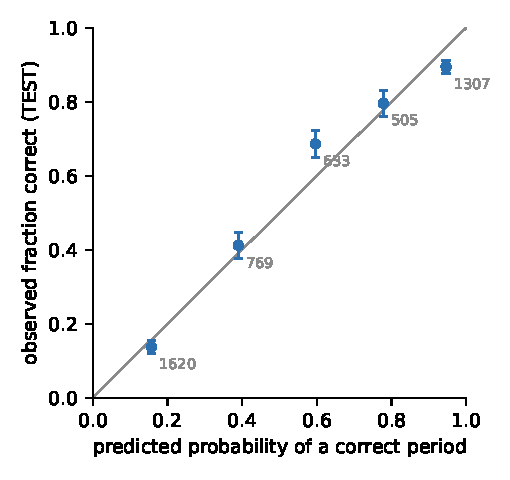
\includegraphics[width=0.95\linewidth]{fig2_reliability.pdf}
\caption{Reliability diagram on TEST for all solutions. Bars are 95\% binomial intervals; numbers give the
count per bin.\label{fig:rel}}
\end{figure}

The confidence threshold was not chosen on TEST. Two null tests use the real Gaia sampling but remove the
rotation. In the \emph{white} test the residuals of the no-rotation model are permuted within seasons; in
the \emph{block} test one-day blocks of residuals are permuted, which keeps correlated systematics. Both
were run on all 32{,}229 solved asteroids without an LCDB period. A noise period matches no catalogue, so
every noise period that passes the threshold ends up among the candidate new periods. The rule is that
the expected noise must stay below 5\% of that list, with the probability scanned in steps of 0.05.

At the TUNE threshold for 80\% precision (0.384), 20.0\% (white) and 18.1\% (block) of the signal-free
asteroids pass (Table~\ref{tab:null}, Figure~\ref{fig:thr}). The rule gives a threshold of 0.80, where 39
(white) and 32 (block) pass. Against the final list of 790 candidates (Section~\ref{sec:new}) that is
4.9\% and 4.1\%, with 95\% Poisson upper limits of 51 and 43, or 6.5\% and 5.4\%. Permuted residuals may
still hold some real signal, so these numbers are estimates rather than strict bounds.

\begin{table}
\centering
\caption{Signal-free asteroids (out of 32{,}229) that reach a given probability in the null tests.}\label{tab:null}
\begin{tabular}{ccc}
\hline
Threshold & White & Block \\
\hline
0.70 & 264 & 248 \\
0.75 & 104 & 108 \\
0.80 & 39 & 32 \\
0.85 & 12 & 8 \\
\hline
\end{tabular}
\end{table}

\begin{figure}
\centering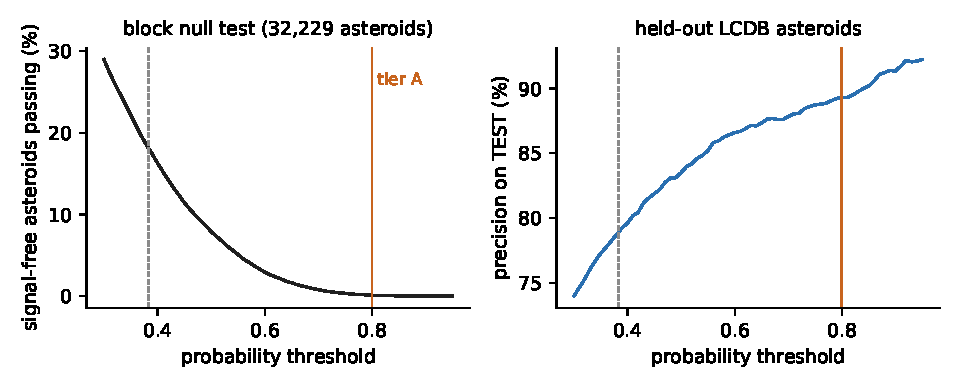
\includegraphics[width=0.95\linewidth]{fig3_threshold.pdf}
\caption{Left: fraction of signal-free asteroids (block null test) that pass, as a function of the
probability threshold. Right: precision on TEST. Dashed line: the TUNE threshold for 80\% precision. Solid
line: the tier-A threshold.\label{fig:thr}}
\end{figure}

Tier~A is probability $\ge0.80$ and period $<100$\,h. Tier~B is probability 0.384--0.80; it is not reliable
for unknown asteroids, because 18--20\% of signal-free asteroids reach it. Periods of 100--1000\,h are
flagged as slow candidates and never treated as confident.

\section{Results}

\subsection{Periods}

6{,}238 periods reach tier~A. On TEST, 1303 of 1459 tier-A periods are correct: 89.3\% (95\% interval
87.6--90.8\%); 90\%, 88\% and 83\% at 2--10, 10--30 and 30--100\,h (Figure~\ref{fig:lcdb}). With tighter
tolerances the figure is 87.9\% within 1\% and 82.7\% within 0.3\%. It depends on the quality of the
reference: 354 of 371 (95.4\%, 92.8--97.1\%) for $U\ge3-$, 935 of 1049 (89.1\%) for $U=2$ and $2+$, and 14 of
39 for $U=2-$; without $U=2-$ it is 90.8\%.

\begin{figure}
\centering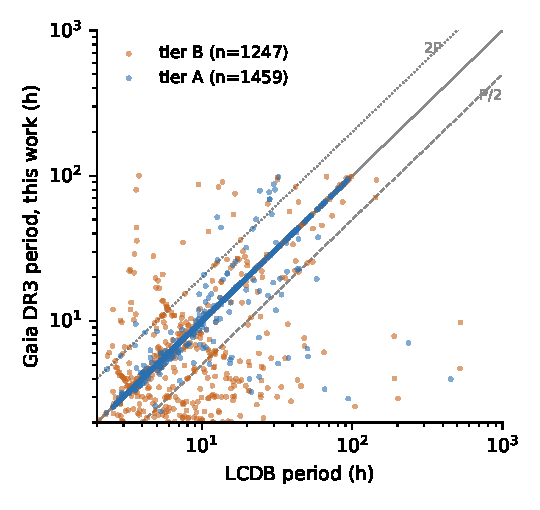
\includegraphics[width=0.95\linewidth]{fig1_lcdb.pdf}
\caption{Period from this work against the LCDB period for TEST asteroids. Blue: tier~A. Orange: tier~B
(probability 0.384--0.80). Lines mark $P$, $2P$ and $P/2$. The off-diagonal scatter includes daily aliases
in the reference periods.\label{fig:lcdb}}
\end{figure}

Of the 156 disagreements, 58 differ from LCDB by exactly one cycle per day in lightcurve frequency, the
typical alias of single-site ground photometry, 6 differ by a factor of two and 92 are other periods. For 38
of them an independent TESS period exists \citep{Vavilov2025}; it agrees with this work in 20 cases, with
LCDB in 3, and with neither in 15.

Table~\ref{tab:lit} compares tier~A with published catalogues. The three Gaia DR3 analyses share the data
and agree at 99--99.6\%; this tests consistency, not accuracy. Among independent surveys, the TESS periods
of \citet{Vavilov2025} agree for 91\%. The ATLAS periods of \citet{Durech2022}, which are not in VizieR and
are therefore not a row of the table, agree for 1{,}088 of 1{,}176 (92.5\%, 90.9--93.9\%), and for 551 of 591
on TEST (93.2\%). In the main disagreement, 72 periods twice theirs, neither side is shown to be right; for
the 36 with an LCDB period, LCDB agrees with this work 31 times. The lower agreement with
\citet{Erasmus2020} and \citet{McNeill2023} reflects those catalogues as much as this one: it rises to 81\%
and 77\% for their own most confident entries, and against LCDB the periods of this work agree more often
than theirs (table note).

\begin{table}
\centering
\caption{Agreement of tier-A periods with published catalogues (within 3\%).}\label{tab:lit}
\begin{tabular}{lccc}
\hline
Catalogue & Data & $n$ & Agree \\
\hline
\citet{Durech2023} & Gaia DR3 & 3564 & 99.6\% \\
\citet{Cellino2024} & Gaia DR3 & 2883 & 99.0\% \\
\citet{MacLennan2026} & Gaia DR3 & 2676 & 99.0\% \\
\citet{Vavilov2025} & TESS & 759 & 91.0\% \\
\citet{Erasmus2020} & ATLAS & 280 & 68.6\% \\
\citet{McNeill2023} & TESS & 863 & 55.0\% \\
\hline
\end{tabular}

\par\smallskip{\footnotesize Agreement measures consistency, not which side is right. It is 81\% for
Erasmus et al.\ entries with confidence $\ge80\%$ ($n=97$) and 77\% for McNeill et al.\ entries with
$CV_{\rm exact}\ge0.9$ ($n=419$). Factor-two relations make up $\le1.2\%$ in every row. For TEST asteroids
also in LCDB, agreement with LCDB (this work vs.\ the catalogue): 373 vs.\ 359 of 411 \citep{Vavilov2025},
111 vs.\ 116 of 146 \citep{Erasmus2020}, and 352 vs.\ 231 of 379 \citep{McNeill2023}.}
\end{table}

The $\chi^2$-curvature errors are too small. Against \citet{Durech2023} the median $|\Delta P/P|$ is
$3.9\times10^{-5}$; the catalogue adds $5.5\times10^{-5}P$ in quadrature, a value chosen so that the median
$|\Delta P|/\sigma$ is 0.67, as for a normal distribution. This compares two analyses of the same data and
does not cover aliasing.

\subsection{Injection--recovery}

I injected synthetic double-peaked lightcurves into the real Gaia sampling of 4{,}000 asteroids without a
known period, with log-uniform periods of 2--100\,h, amplitudes of 0.1--0.6\,mag scaled by 0.5--1 per
season, and a random sense with the phase following $\lambda_{\rm PAB}$. The noise was either the object's
own permuted residuals (pessimistic) or Gaussian at the quoted errors (optimistic). Tier~A is precise under
both: 96.5\% (109/113) and 99.3\% (567/571) of its periods are correct, with no $P/2$ or $2P$ errors, and the
sense is correct for 96--97\% of the correct periods. Because the injected signals have the model's own form
and an exact PAB shift, these figures are upper limits; the TEST and survey comparisons are the realistic
ones. Completeness is low, 2.7\% and 14\%, against 10.5\% of real unknown asteroids that reach tier~A, and
no amplitude below 0.2\,mag is recovered. Tier~A is a high-precision, low-completeness selection and should
not be used for population statistics without a selection-function correction.

\subsection{Spin senses}\label{sec:spin}

The sense $s$ was compared with the hemisphere of published poles, excluding poles within $20^\circ$ of the
ecliptic and pole pairs in opposite hemispheres. It agrees for 3473 of 3535 asteroids (98.2\%, 97.8--98.6\%)
with \citet{Durech2023}, which uses the same data; the 62 errors are nearly symmetric, 34 prograde called
retrograde and 28 the reverse. It agrees for 3802 of 3899 (97.5\%) with DAMIT \citep{Durech2010}, 372 of 394
(94.4\%) with DAMIT asteroids not in \citet{Durech2023}, and 374 of 388 (96.4\%, 94.0--97.8\%) with the poles
that \citet{Durech2020} derived from ATLAS photometry alone, 130 of 137 for those not in \citet{Durech2023}.

Accuracy depends on pole latitude, as expected from Section~\ref{sec:model}. Against \citet{Durech2023} it is 98.7\%
(3326/3371) for $|\beta|\ge40^\circ$, 78\% (86/110) for $20^\circ\le|\beta|<40^\circ$ and 9 of 16 below
$20^\circ$. Tier~A favours poles far from the ecliptic: among asteroids with poles in \citet{Durech2023},
$|\beta|<30^\circ$ for 1.7\% of tier-A members and 15.5\% of the others, probably because such poles give
large amplitudes in every season. Most tier-A senses therefore belong to high-$|\beta|$ poles, but the
accuracy of an individual sense with an unknown pole cannot be guaranteed.

1{,}447 tier-A asteroids have no pole in \citet{Durech2023}, DAMIT, \citet{Cellino2024}, \citet{MacLennan2026},
\citet{Durech2020} or \citet{Durech2016}; for them the sense of rotation is new. The SsODNet spin compilation
was not searched.

Tier~A has 3{,}677 retrograde and 2{,}561 prograde rotators (59\% retrograde). This excess is mostly a
selection effect: applying the tier-A selection to the poles of \citet{Durech2023} gives 54\% retrograde
among tier-A members against 40\% among the others.

\subsection{Yarkovsky segregation in families}

The Yarkovsky drift moves prograde rotators outward and retrograde ones inward, so the two senses lie on
opposite sides of a family's V-shape \citep{Vokrouhlicky2015}. This has been shown with modelled poles
\citep{Hanus2013,Hanus2018,Kryszczynska2013} and, from Gaia DR3, by \citet{Durech2023} in Eos, Eunomia,
Themis and Koronis. Here it serves as a test of the senses and is quantified with a permutation null.

I used AstDyS family membership and synthetic proper elements \citep{Knezevic2003,Milani2014}, with the
proper $a$ of the namesake as each family's centre $a_c$. A member is consistent if it is prograde and
outside the centre, or retrograde and inside it. The null hypothesis keeps each family's mix of senses and
its positions and breaks only the link between them, so I permuted the senses within each family 20{,}000
times. 1{,}753 of 2{,}345 tier-A members (74.8\%) are consistent, against $52.4\pm0.9\%$ under the null
($z=24.7$; no permutation reaches the observed value; odds ratio 9.1). Without Eos, which dominates, the
fraction is 71.1\%. With $d=|a-a_c|\,10^{-0.2H}$, a distance in units of the V-shape that removes the $1/D$
dependence of the drift, normalised by each family's median, the fraction rises from 58\% ($d<0.5$) to 75\%
(0.5--1), 82\% (1--2) and 82\% ($d\ge2$). With the median $a$ of all members as centre it is 71.3\%; for the
912 members without a pole in \citet{Durech2023} it is 73.6\%. The largest families show it clearly: (221)
Eos 86\% of 578, (24) Themis 81\% of 184, (15) Eunomia 79\% of 294, (158) Koronis 78\% of 184
(Figure~\ref{fig:yark}). Two smaller families, (93) Minerva and (375) Ursula, show the opposite pattern,
which may reflect a namesake far from the family centre or interlopers.

For the 1{,}530 members with published poles, the senses of this work are correct for 98.2\%, almost
equally on the two sides (98.6\% and 97.0\%), and give a consistent fraction of 75.4\% against 75.8\% with
the published poles. The 74.8\% therefore measures the segregation itself, for a subset that favours high
amplitudes and high $|\beta|$, where the drift is fastest; it does not describe complete families.

\begin{figure}
\centering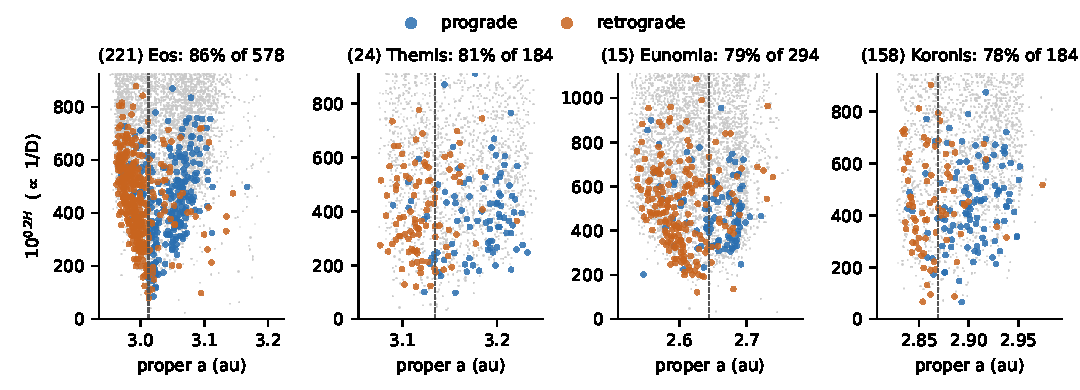
\includegraphics[width=0.95\linewidth]{fig4_yarkovsky.pdf}
\caption{Four families in proper semimajor axis against $10^{0.2H}\propto1/D$. Grey: all AstDyS members.
Blue: prograde; orange: retrograde (tier~A, this work). Dashed line: the namesake. Each title gives the
fraction of members on the side the Yarkovsky effect predicts.\label{fig:yark}}
\end{figure}

\subsection{Disputed LCDB periods}

I selected tier-A asteroids whose LCDB V4.0 period disagrees with this work and where either an independent
survey supports this work and none supports LCDB \citep{Vavilov2025,McNeill2023,Erasmus2020}, or at least
two other Gaia DR3 analyses support this work. This gives 117 asteroids, 32 of them exact daily aliases and
14 differing by a factor of two. In the 2023 LCDB revision distributed by the JPL Small-Body Database, 9 of
the 117 had already been revised by others to the value found here, an independent sign that the selection
finds real errors.

The other 108 are still in the LCDB, in two groups of different weight. The 39 in Table~\ref{tab:lcdb39}
disagree with independent survey data: a TESS or ATLAS period agrees with this work and none agrees with
LCDB. They are not proven errors. The supporting surveys are less accurate than LCDB on average
(Table~\ref{tab:lit}), only 17 of the 39 are supported by two surveys, and 13 are factor-two cases, where
sparse surveys share the same ambiguity. The TESS comparison above suggests that roughly half of such
disagreements are LCDB errors. The six with $U\ge3-$ deserve a closer look first. The other 69 are only
\emph{flagged}: they rest on Gaia DR3 analyses, which share the sampling and its aliases, and call for
re-observation rather than correction. The full list of 117, with the supporting catalogues, is part of the
data release.

\begin{table*}
\centering
\caption{The 39 LCDB V4.0 periods that disagree with independent survey data. Relation: d, daily alias; 2,
factor of two; o, other. Survey periods: V, \citet{Vavilov2025} (TESS); M, \citet{McNeill2023} (TESS); E,
\citet{Erasmus2020} (ATLAS).}\label{tab:lcdb39}
\footnotesize
\begin{tabular}{rrcrcl}
\hline
Number & $P_{\rm LCDB}$ (h) & $U$ & $P$ this work (h) & Rel. & Survey periods (h) \\
\hline
1040 & 59.2 & 2 & 37.7324 & o & 37.736$^{\rm V}$, 37.679$^{\rm M}$ \\
1940 & 6.953 & 3 & 6.5954 & o & 6.596$^{\rm V}$, 6.597$^{\rm M}$ \\
2884 & 14.31 & 2+ & 35.5264 & o & 35.522$^{\rm E}$ \\
2933 & 13.482 & 2 & 13.0343 & o & 13.033$^{\rm V}$, 13.032$^{\rm M}$ \\
3422 & 2.91 & 3 & 3.2183 & o & 3.218$^{\rm V}$, 3.218$^{\rm M}$ \\
3813 & 12.3 & 3- & 11.7155 & o & 11.713$^{\rm E}$ \\
3867 & 28.035 & 2 & 51.0687 & o & 51.031$^{\rm V}$, 51.081$^{\rm M}$ \\
4488 & 24.25 & 2 & 78.7370 & o & 78.640$^{\rm E}$ \\
5702 & 9.5 & 2+ & 10.3314 & o & 10.333$^{\rm E}$ \\
8397 & 3.9 & 3- & 4.4223 & o & 4.422$^{\rm V}$, 4.422$^{\rm M}$ \\
8744 & 5.199 & 2 & 5.3677 & o & 5.367$^{\rm E}$ \\
8847 & 5.75 & 2 & 5.2301 & o & 5.229$^{\rm E}$ \\
10338 & 10.55 & 2 & 13.4825 & d & 13.482$^{\rm E}$ \\
10816 & 14.12 & 2 & 28.4494 & 2 & 28.461$^{\rm E}$ \\
11087 & 4.5369 & 3 & 6.2802 & o & 6.281$^{\rm V}$ \\
13894 & 5.9 & 2 & 5.4779 & o & 5.477$^{\rm V}$, 5.475$^{\rm M}$, 5.478$^{\rm E}$ \\
14376 & 5.614 & 3 & 5.8485 & o & 5.849$^{\rm V}$, 5.848$^{\rm M}$ \\
17079 & 4.18 & 2+ & 3.8586 & d & 3.859$^{\rm E}$ \\
17390 & 3.47535 & 2 & 6.9528 & 2 & 6.948$^{\rm V}$ \\
17627 & 42.462 & 2 & 40.6427 & o & 40.619$^{\rm E}$ \\
20623 & 19.936 & 2 & 20.5829 & o & 20.562$^{\rm V}$ \\
23795 & 9.473 & 2 & 11.8136 & d & 11.823$^{\rm V}$, 11.810$^{\rm M}$ \\
26216 & 23.9952 & 2 & 4.1208 & o & 4.111$^{\rm V}$ \\
28754 & 7.0243 & 2 & 14.0457 & 2 & 14.048$^{\rm V}$, 14.070$^{\rm M}$ \\
32358 & 21.82 & 2 & 43.0516 & 2 & 43.252$^{\rm V}$ \\
34131 & 2.32495 & 2 & 4.6472 & 2 & 4.651$^{\rm V}$ \\
37534 & 5.293 & 2 & 5.0942 & o & 5.096$^{\rm V}$ \\
43089 & 36.2149 & 2 & 5.2126 & o & 5.208$^{\rm V}$ \\
45659 & 3.848 & 2 & 3.5608 & d & 3.557$^{\rm V}$, 3.561$^{\rm M}$ \\
48694 & 94.0207 & 2 & 2.9181 & o & 2.916$^{\rm V}$ \\
53324 & 3.59911 & 2 & 7.2018 & 2 & 7.184$^{\rm V}$ \\
53396 & 1.41998 & 2 & 2.8409 & 2 & 2.840$^{\rm V}$ \\
55098 & 5.71996 & 2 & 11.4198 & 2 & 11.360$^{\rm V}$ \\
55543 & 2.86191 & 2 & 5.7249 & 2 & 5.722$^{\rm V}$, 5.725$^{\rm M}$ \\
57674 & 5.63622 & 2 & 11.2749 & 2 & 11.266$^{\rm V}$, 11.278$^{\rm M}$ \\
65441 & 3.55382 & 2 & 7.1060 & 2 & 7.106$^{\rm V}$, 7.107$^{\rm M}$ \\
91070 & 4.16574 & 2 & 8.3317 & 2 & 8.331$^{\rm V}$, 8.333$^{\rm M}$ \\
91256 & 1.43726 & 2 & 2.8745 & 2 & 2.875$^{\rm V}$, 2.874$^{\rm E}$ \\
109214 & 6.8107 & 2 & 5.7524 & o & 5.749$^{\rm V}$, 5.761$^{\rm M}$ \\
\hline
\end{tabular}
\end{table*}

\subsection{Candidate new periods}\label{sec:new}

942 tier-A asteroids have no LCDB period with $U\ge2-$ and no period in the six catalogues of
Table~\ref{tab:lit}. I searched further: DAMIT; about 180 VizieR tables with rotation periods (5.0\,M rows),
with units from the table metadata and non-rotation periods excluded; the Minor Planet Bulletin, volumes
50--53; the ATLAS periods of \citet{Durech2022}; the current JPL SBDB, which carries the October 2023 LCDB
revision; and the SsODNet best-estimate table ssoBFT \citep{Berthier2023}, in a snapshot of 22 September
2026. The snapshot contains 92\% of the \citet{Durech2022} periods for asteroids without an LCDB period, so
a few published periods may still be missed. Behrend's Geneva pages and ZTF period catalogues outside
VizieR were not searched.

152 of the 942 (16.1\%) have a period in one of these sources, including five whose LCDB entry has
$U=1$ or only a lower limit. For the 66 of them with a prior period from the last three sources and
$U\ne1$, this work agrees in 48 (73\%, 61--82\%), against 93.9\% for the rest of tier~A compared with the
same sources; against \citet{Durech2022} alone the figures are 35 of 46 (76\%) and 93.2\%. Most
disagreements are simple relations (7 periods twice the prior one, 6 daily aliases, 2 at 3/2). Periods from
the same Gaia data \citep{Durech2023,Cellino2024,MacLennan2026} count against novelty but never as
confirmation.

The remaining 790 are candidate new periods: 617 at 2--10\,h, 116 at 10--30\,h and 57 at 30--100\,h. Two
estimates bracket their reliability. TEST precision reweighted to the candidates' distribution of
probability, amplitude and number of transits is 87\%. Agreement with prior periods for the 66 comparable
asteroids is 73\%. The two differ, probably because asteroids without published periods are harder cases
than the covariates capture. Between about 60\% and 87\% of the 790 periods are therefore expected to be
correct; noise accounts for 4--5\%, and most of the rest are likely harmonics or aliases of the true period.
For each candidate the catalogue gives the second-best period. The list is a set of targets for
dense-lightcurve observers, biased to large amplitudes, high $|\beta|$ and periods above 2\,h; it is not a
population sample. An earlier release of the catalogue listed 861 candidates before the last three sources
were searched.

Of the 42 candidates of the pilot \citep{Tropynin2026a}, 34 remain new; 4 are probably twice the pilot
period, 3 now prefer slow solutions, and one, 11857, has a matching period in \citet{Durech2022}.

\section{Limitations and plans for Gaia DR4}

Periods below 2\,h are not searched, and tumblers fall outside a single-period model. The doubling rule
based on the ratio of the two harmonics is a heuristic. When the Fourier fit is at half the rotation
period, the PAB term should enter with a factor 2; a variant that also tries this changed TEST precision
only from 89.3\% to 89.7\% and was not adopted. The probability is slightly overconfident in its top bin.
Completeness is low below 0.3\,mag and nil below 0.2\,mag, the injection test does not model aspect-dependent
amplitudes, and spin senses are reliable mainly for poles far from the ecliptic.

DR4 will cover about 66 months. For it, I plan to fit the sidereal period and the pole jointly on a coarse
pole grid, with a model-based test of $P$ against $2P$, injections from DAMIT shape models with realistic
poles, and a recalibrated probability. Thresholds and null tests can then be reused unchanged, so that
results can be released within a day.

\section{Conclusions}

From Gaia DR3 sparse photometry alone, 6{,}238 asteroid rotation periods reach a tier whose precision is
89\% against held-out LCDB periods and 92--93\% against independent ATLAS periods. Each comes with a
probability and a spin sense; the senses agree with independent ATLAS poles for 96\% and reproduce the
Yarkovsky segregation in families. For asteroids without a published period, the error rate is higher than
for known ones, and this paper measures by how much: 790 candidate new periods carry an estimated 4--5\%
noise, and a further 8--36\% are probably harmonics or aliases. Observers can use the candidate list and the 39
LCDB periods contradicted by survey data as target lists; modellers can use the 1{,}447 new senses with the
latitude caveat. The same pipeline, thresholds and null tests are ready for Gaia DR4.
